\documentclass[12pt, a4paper]{article}
\usepackage{../../../myconfig} % Gọi file cấu hình từ ngoài gốc vào

% ==========================================
% BẮT ĐẦU NỘI DUNG TÀI LIỆU
% ==========================================
\begin{document}

% Truyền 3 tham số: {Nhãn cam} {Chữ to chính giữa} {Chữ ở góc phải Header}
\titlebox{Chủ đề: Hàm số}{BTDD ứng dụng khảo sát đồ thị hàm số}{Hàm số: Ứng dụng đồ thị}

% --- CÂU 1 ---
\questionTrueFalse{12}{1}{Chi phí nhiên liệu của một chiếc tàu chạy trên sông được chia làm hai phần. Phần thứ nhất không phụ thuộc vào vận tốc và bằng 600 nghìn đồng trên 1 giờ. Phần thứ hai tỉ lệ thuận với lập phương của vận tốc, khi \( v = 12 \, (\text{km/giờ}) \) thì phần thứ hai bằng 45 nghìn đồng/giờ. Xét tính đúng sai của các mệnh đề sau:}{
    \textbf{a)} & Khi vận tốc \( v = 12 \, (\text{km/giờ}) \) thì chi phí nguyên liệu cho phần thứ nhất trên 1 km đường sông là 50000 đồng.
    & \textcolor{amberorange}{$\bigcirc$} & \textcolor{amberorange}{$\bigcirc$} \\ \hline
    
    \textbf{b)} & Hàm số xác định tổng chi phí nguyên liệu trên 1 km đường sông với vận tốc \( x \, (\text{km/h}) \) là  
    \[f(x) = \dfrac{600}{x} + \dfrac{5}{192}x^3 \quad (\text{đơn vị: nghìn đồng}).\]
    & \textcolor{amberorange}{$\bigcirc$} & \textcolor{amberorange}{$\bigcirc$} \\ \hline
    
    \textbf{c)} & Khi vận tốc \( v = 24 \, (\text{km/giờ}) \) thì tổng chi phí nguyên liệu trên 1 km đường sông là 40000 đồng.
    & \textcolor{amberorange}{$\bigcirc$} & \textcolor{amberorange}{$\bigcirc$} \\ \hline
    
    \textbf{d)} & Vận tốc của tàu để tổng chi phí nguyên liệu trên 1 km đường sông nhỏ nhất là \( v = 20 \, (\text{km/giờ}). \)
    & \textcolor{amberorange}{$\bigcirc$} & \textcolor{amberorange}{$\bigcirc$} \\
}

% --- CÂU 3 ---
\questionTrueFalse{15}{2}{Tại trang trại bò của bác Ba, người ta thống kê số lượng lít sữa thu được mỗi tuần sau \( t \) tuần (\( t \geq 1 \)) và thu được bảng dữ liệu sau:  

\begin{table}[h!]
\centering
\renewcommand{\arraystretch}{2.0} % Tăng khoảng cách dòng để các phân số không bị dính vào đường kẻ
\begin{tabular}{|c|c|c|c|c|c|}
\hline
$t$ (tuần) & 5 & 10 & 15 & 20 & 25 \\ \hline
\begin{tabular}[c]{@{}c@{}}Lượng sữa \ (lít)\end{tabular} & 130 & $\dfrac{2040}{13}$ & $\dfrac{1520}{9}$ & $\dfrac{4040}{23}$ & 180 \\ \hline
\end{tabular}
\end{table}

Biết rằng hàm số mô tả lượng sữa thu được trong trang trại có dạng \( y = \dfrac{at + b}{ct + d} \) (\( ad - bc \neq 0, c \neq 0 \)).}{
    \textbf{a)} & Hàm số mô tả lượng sữa thu được trong trang trại bò của bác Ba sau \( t \) tuần có dạng \( y = \dfrac{200t + 40}{t + 3} \).
    & \textcolor{amberorange}{$\bigcirc$} & \textcolor{amberorange}{$\bigcirc$} \\ \hline
    
    \textbf{b)} & Tại thời điểm tuần thứ 12, lượng sữa thu được là 162 lít.
    & \textcolor{amberorange}{$\bigcirc$} & \textcolor{amberorange}{$\bigcirc$} \\ \hline
    
    \textbf{c)} & Lượng sữa thu được trong trang trại không vượt quá 190 lít.
    & \textcolor{amberorange}{$\bigcirc$} & \textcolor{amberorange}{$\bigcirc$} \\ \hline
    
    \textbf{d)} & Kể từ tuần 8, lượng sữa thu được trong trang trại vượt quá 150 lít.
    & \textcolor{amberorange}{$\bigcirc$} & \textcolor{amberorange}{$\bigcirc$} \\
}

% --- CÂU 10 ---
\questionShortAnswer{15}{3}{Anh Huy tham dự giải "Đi bộ vì cuộc sống xanh" năm 2026. Quãng đường anh đi được biểu diễn bằng hàm số \( s(t) = at^3 + bt^2 + ct + d \) với \( a \neq 0 \) có đồ thị như hình bên. Trong đó \( t \) được tính bằng giờ \( (0 \leq t \leq 3) \), \( s \) là quãng đường tính bằng \( km \). Khi đó vận tốc tối đa của anh Huy đạt được trong quá trình đi bộ là bao nhiêu \( km/h \)?
\begin{center}
\begin{tikzpicture}[>=latex, scale=0.5]
    % Vẽ hệ trục
    \draw[->] (-2,0) -- (6,0) node[below] {$t$};
    \draw[->] (0,-1) -- (0,12) node[right] {$s$};
    \node[below left] at (0,0) {$O$};
    
    % Đánh dấu các mốc
    \draw (2,0.1) -- (2,-0.1) node[below] {$2$};
    \draw (3,0.1) -- (3,-0.1) node[below] {$3$};
    \draw (0.1,54/5) -- (-0.1,54/5) node[left] {$\dfrac{54}{5}$};
    \draw (0.1,8)--(-0.1,8) node[left] {$8$};
    % Vẽ đồ thị hàm số bậc 3
    \draw[ultra thick, samples=100, domain=-1:4.55] 
       plot (\x, {-4/5*\x*\x*\x + 18/5*\x*\x});
    
    \draw[dashed] (2,0) -- (2,8) -- (0,8);
    \draw[dashed] (3,0) -- (3,54/5) -- (0,54/5);
    
\end{tikzpicture}
\end{center}}

% --- CÂU 13 ---
\questionShortAnswer{15}{4}{Một máy bay trình diễn có đường bay gắn với hệ trục \( Oxy \) được mô phỏng như hình vẽ, trục \( Ox \) gắn với mặt đất. Đường bay có dạng là một phần của đồ thị hàm số phân thức bậc hai trên bậc nhất \( y = f(x) \) có đường tiệm cận đứng là \( x = 2 \). \( G \) là giao điểm của đường tiệm cận xiên của đồ thị hàm số \( y = f(x) \) và trục \( Ox \) được gọi là điểm giới hạn. Biết rằng máy bay xuất phát tại vị trí \( A \) cách gốc tọa độ \( O \) một khoảng 2,5 đơn vị và máy bay khi ở vị trí cao nhất cách điểm xuất phát 1,5 đơn vị theo phương song song với trục \( Ox \) và cách mặt đất 4,5 đơn vị. Vị trí máy bay tiếp đất cách điểm giới hạn một khoảng bằng bao nhiêu?

\begin{center}
\begin{tikzpicture}[>=latex, scale=0.8]
    % Vẽ hệ trục
    \draw[->] (-3,0) -- (12,0) node[below] {$x$};
    \draw[->] (0,-1) -- (0,6) node[right] {$y$};
    \node[below left] at (0,0) {$O$};
    
    % Đánh dấu các mốc
    \draw (2,0.1) -- (2,-0.1) node[below left] {$2$};
    
    % Vẽ đồ thị hàm số
    \draw[thick, samples=100, domain=2.44:10.8] 
        plot (\x, {(-2*\x*\x + 25*\x - 50)/(2*\x - 4)});
    \draw[dashed, samples=100, domain=3:11.2] 
        plot (\x, {-\x + 10.5});
    % Đường tiệm cận
    \draw[dashed] (2,-1) -- (2,6) ;
    
    
    % Điểm A, G
    \fill (2.5,0) circle (3pt) node[above right] {$A$};
    \fill (4,4.5) circle (3pt) node[above] {$B$};
    \fill (10.5,0) circle (3pt) node[above] {$G$};
\end{tikzpicture}
\end{center}}

\end{document}
